\subsection{Independent curated labels (OmniPath, miRTarBase removed): CNN above chance, but not above site count or expression}
The miRTarBase and Enrichr analyses share one curation source. OmniPath aggregates several (script and results: \texttt{omnipath\_independent}; hermetic tests), so we kept only interactions whose sources exclude miRTarBase (2,795 of 11,240; ncRDeathDB, miRecords, miR2Disease, miRDeathDB, SIGNOR) and scored them inside each miRNA's CLIP universe of non-conserved seed-match genes. The site-count, expression and label-permutation controls were fixed before scoring.
Gates passed: 13 miRNAs have at least five positives (bar 10), and the median permutation-mean CNN AUROC is 0.504. The CNN is above chance (H1: 11/2, $p=0.011$, median AUROC 0.566), but it does not beat site count (H2: 8/5, $p=0.291$, median 0.572) and loses to HEK293 expression (H3: 3/10, median 0.689; Figure~\ref{fig:omnipath}). This matches the Enrichr replication on a label set that shares no miRTarBase rows: curated low-throughput targets favour expressed genes, and whatever the CNN adds over counting seed sites is not detectable with 5--29 positives per miRNA.
\begin{figure}[h]\centering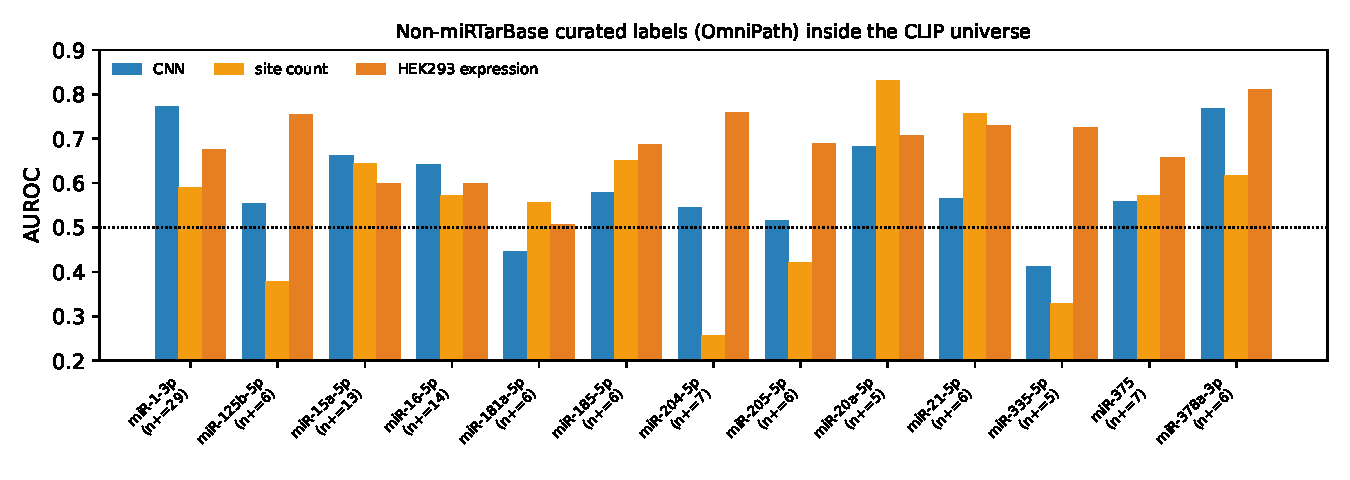
\includegraphics[width=0.95\linewidth]{figs/fig_omnipath.pdf}
\caption{Per-miRNA AUROC on OmniPath interactions with miRTarBase-sourced rows removed, for the CNN, site count and HEK293 expression.}\label{fig:omnipath}\end{figure}
